\newpage
\cleardoublepage

\chapter{Εισαγωγή}
\label{chap:1}
% Η πρώτη σελίδα κάθε κεφαλαίου ορίζεται με απλό στυλ επικεφαλίδων και αρίθμησης σελίδων
\thispagestyle{plain}


\section{Περιγραφή του Προβλήματος }
\label{sec:1.1}
Η παρούσα διπλωματική πραγματεύεται την ανίχνευση της χρήζουσας θεραπείας Διαβητικής Αμφιβληστροειδοπάθειας(referable Diabetic Retinopathy). Η Διαβητική Αμφιβληστροειδοπάθεια (Diabetic Retinopathy) είναι μία ασθένεια που χαρακτηρίζεται από βλάβες του αμφιβληστροειδούς, λόγω του Σακχαρώδη Διαβήτη.

Ο Σακχαρώδης Διαβήτης προσβάλλει  περισσότερο από 415 εκατομμύρια ανθρώπους παγκοσμίως ή 1 στους 11 ενήλικες, ενώ ο αριθμός των ασθενών προβλέπεται να αυξηθεί στους 642 εκατομμύρια, μέχρι το 2040 \cite{Gargeya}\cite{Wang}. Πάνω από το ένα τρίτο των ατόμων που πάσχουν από Σακχαρώδη Διαβήτη, αναμένεται να εμφανίσουν κάποια μορφή DR \cite{Congdon}.

Η διάγνωση της DR γίνεται από οφθαλμιάτρους  με απευθείας εξέταση ή με χρήση έγχρωμων εικόνων του αμφιβληστροειδούς. Η καθιερωμένη διαδικασία διάγνωσης της ασθένειας είναι ακριβή και απαιτεί εξειδικευμένους οφθαλμιάτρους \cite{Nayak}.

Επίσης, το 75$\%$ των ασθενών με DR ζουν σε χώρες με μικρό κατά κεφαλήν εισόδημα που η έλλειψη καταρτισμένων ιατρών και υποδομών είναι μεγάλη, ενώ συγχρόνως πολλοί ασθενείς δεν έχουν την οικονομική δυνατότητα επίσκεψης στον οφθαλμίατρο \cite{Guariguata}\cite{Wang}.




\section{Στόχοι της Εργασίας}
\label{sec:1.2}
Στόχος της εργασίας είναι η υλοποίηση ενός αλγορίθμου για την αυτόματη ανίχνευση της rDR με χρήση βαθιών συνελικτικών δικτύων. Συνδυαστικά με τον παραπάνω αλγόριθμο προβλέπεται η δημιουργία ενός συστήματος οπτικοποίησης των περιοχών που εντοπίζεται η ασθένεια από το νευρωνικό.


Το παραπάνω σύστημα προβλέπεται να ενσωματωθεί στη διαδικασία της διάγνωσης. Ένας πιθανός τρόπος ενσωμάτωσης είναι ο εξής: Εικόνες του αμφιβληστροειδούς θα λαμβάνονται από εκπαιδευμένο προσωπικό(όχι απαραίτητα εξειδικευμένο οφθαλμίατρο ή γιατρό) και στη συνέχεια με τον αυτόματο αλγόριθμο που υλοποιήθηκε θα προβλέπεται αν ο ασθενής έχει rDR ή όχι ενώ ταυτόχρονα θα οπτικοποιούνται οι περιοχές στις οποίες το νευρωνικό εντοπίζει την rDR. Τέλος, τα περιστατικά με rDR θα παραπέμπονται σε ειδικό ιατρό.

Έτσι, μειώνεται ο συνολικός χρόνος διάγνωσης αφού μόνο τα περιστατικά με rDR θα παραπέμπονται στον εξειδικευμένο οφθαλμίατρο ενώ παράλληλα η οπτικοποίηση των περιοχών στις οποίες το νευρωνικό εντοπίζει την ασθένεια θα αποτελεί μία κατευθυντήρια γραμμή για τον ιατρό ώστε να πετυχαίνει εγκυρότερη και ταχύτερη διάγνωση.





\section{Διαβητική Αμφιβληστροειδοπάθεια }
\label{sec:1.3}
Η DR σύμφωνα με την International Clinical Diabetic Retinopathy(ICDR) μπορεί να ταξινομηθεί στα παρακάτω στάδια: no, mild, moderate, severe, και proliferative. Ωστόσο, απαντώνται διάφορα συστήματα αξιολόγησης της ασθένειας ενώ πολλές φορές υπάρχει ασυμφωνία των ειδικών πάνω στην ερμηνεία των αποτελεσμάτων \cite{Lin}.

Ως rDR ορίζεται η ασθένεια από το στάδιο Moderate και πάνω, δηλαδή moderate, severe και proliferative DR ή/και ύπαρξη οιδήματος της ωχράς κηλίδας. Το οίδημα της ωχράς κηλίδας δεν θα μελετηθεί στην παρούσα διπλωματική. Οι περισσότερες οδηγίες αναφέρουν ετήσια οφθαλμολογική παρακολούθηση για τα άτομα με Σακχαρώδη Διαβήτη που δεν εμφανίζουν DR ή εμφανίζουν mild DR\cite{Congdon}. Ενώ σε περίπτωση moderate DR συνίσταται η επανάληψη της εξέτασης  σε ένα εξάμηνο. Τέλος, για αυτούς που θα διαγνωστούν με severe ή proliferative  DR η εξέταση θα πρέπει να επαναληφθεί μέσα σε λίγες εβδομάδες\cite{Gulshan}.

Στα πρώτα στάδια της ασθένειας, πιθανότητα να μην υπάρχουν συμπτώματα για τον ασθενή. Ωστόσο, όσο η κατάσταση επιδεινώνεται  μπορούν να παρατηρηθούν τα εξής: θολή όραση, σκοτεινές περιοχές, στίγματα που ακολουθούν τις κινήσεις του οφθαλμού, θάμβος οράσεως που η έντασή του παρουσιάζει διακύμανση, δυσκολία στην αντίληψη του χρώματος και ολική  τύφλωση\cite{Giraddi}. Η DR αποτελεί κυρίαρχο, δυνάμενο να προβλεφθεί, παράγοντα τύφλωσης\cite{Ciulla}. Ενδεικτικά, παρουσιάζεται η εικόνα \ref{figure:drSymptoms}, ώστε να γίνει αντιληπτό πως επιδρά η ασθένεια στην όραση τους ασθενούς. 

\begin{figure}[!h]
    \centering
      
\includegraphics[width=1\linewidth]{drSymptoms.jpg} \caption{(α')Οπτική ενός υγιούς ατόμου (β')Οπτική ενός ατόμου με Διαβητική Αμφιβληστροειδοπάθεια}
\label{figure:drSymptoms}  
\end{figure}

Όσον αφορά τη διάγνωση, σημαντικότερα σημάδια της ασθένειας αποτελούν τα μικροανευρίσματα, τα νεοαγγεία, οι αιμορραγίες, τα σκληρά  εξιδρώματα και οι βαμβακόμορφες κηλίδες \cite{Nayak}\cite{Acharya}. Στην εικόνα \ref{figure:signs} επισημαίνονται τα συμπτώματα της ασθένειας.


\begin{figure}[!h]
    \centering
      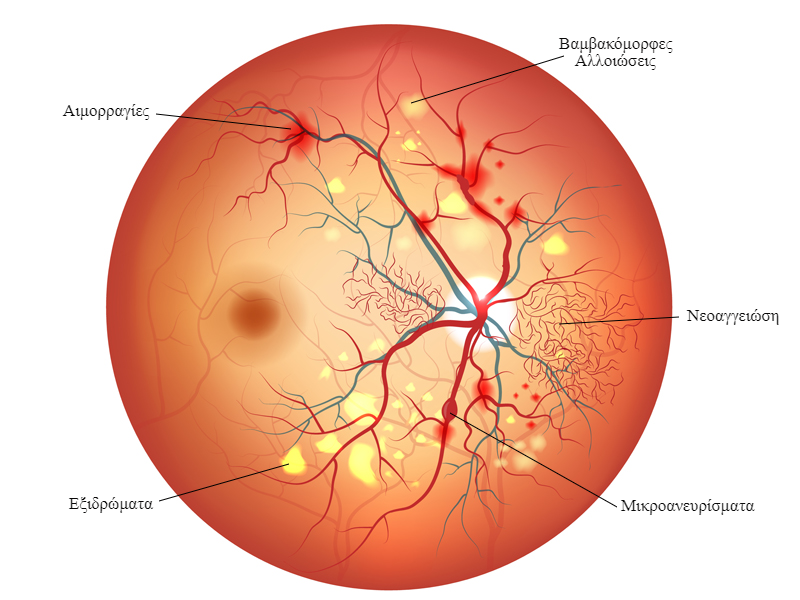
\includegraphics[width=0.7\linewidth]{signs.png} \caption{Συμπτώματα της Διαβητικής Αμφιβληστροειδοπάθειας}
       \label{figure:signs}    
  \end{figure}



\section{Διάρθρωση της Εργασίας}
Tο \textbf{Κεφάλαιο 1} αποτελεί την εισαγωγή στη διπλωματική εργασία. Δίνεται ενδεικτικά μία περιγραφή του προβλήματος. Στη συνέχεια, αναλύεται ο στόχος της διπλωματικής και περιγράφεται η ασθένεια της Διαβητικής Αμφιβληστροειδοπάθειας. 

Στο \textbf{Κεφάλαιο 2} δίνονται συνοπτικά οι δύο  σημαντικότερες  προσεγγίσεις που απαντώνται στη βιβλιογραφία για την αυτόματη ανίχνευση της rDR ή της DR και παρουσιάζονται κάποιες σχετικές εργασίες.

Στο \textbf{Κεφάλαιο 3} εξηγούνται σημαντικές έννοιες και δίνονται πληροφορίες για τα τεχνητά νευρωνικά δίκτυα, τα συνελικτικά νευρωνικά δίκτυα και τις Μηχανές Διανυσμάτων Υποστήριξης. Επιπλέον, γίνεται αναφορά στο νευρωνικό Inception V3 και περιγράφονται μερικές από τις τεχνικές σχεδίασης του. Τέλος, παρουσιάζονται τα εργαλεία που χρησιμοποιήθηκαν.

Στο \textbf{Κεφάλαιο 4} παρουσιάζονται συνοπτικά τα σύνολα δεδομένων Kaggle και Messidor 2. Επίσης, παρουσιάζεται ο αλγόριθμος που χρησιμοποιήθηκε για τη μείωση των διαστάσεων των εικόνων.

Στο \textbf{Κεφάλαιο 5} παρουσιάζονται οι μέθοδοι
που απέδωσαν τα καλύτερα αποτελέσματα για την  ανίχνευση της rDR ενώ παράλληλα γίνεται μία  αναφορά σε προσπάθειες που επέφεραν ισάξια ή κατώτερα αποτελέσματα.

Στο \textbf{Κεφάλαιο 6} γίνεται αναφορά στις μετρικές που επιλέχθηκαν για την αξιολόγηση της παρούσας διπλωματικής και περιγράφεται ο τρόπος υπολογισμού τους.

Στο \textbf{Κεφάλαιο 7} παρουσιάζονται και σχολιάζονται τα αποτελέσματα των καλύτερων μεθόδων. Επίσης, εξηγείται η μέθοδος που ακολουθήθηκε για την οπτικοποίηση των περιοχών, που σύμφωνα με το νευρωνικό, εντοπίζεται η ασθένεια και δίνονται κάποια παραδείγματα οπτικοποίησης. Τέλος, γίνεται αναφορά σε μελλοντικές επεκτάσεις.


